\section{Evaluation}
\label{sec:performance}

In this section, we evaluate the performances of our designs from three aspects: influence, robustness, and effectiveness. With respect to influence, we conducted analysis on how many apps on the NeuroSky App Store are vulnerable to our attacks. As for robustness, we probed into the circumstances of how effective our attacks are based on different attacking environments. Lastly, we demonstrated the effectiveness by showing the accuracy of our inference attack and comparing the results with other well-known and widely-used machine learning algorithms.

\subsection{Influence of the Attacks}
In this subsection, we study the numbers of apps in the NeuroSky App store that are affected by our attacks. So far, the NeuroSky App store contains 156 apps, with 31 free apps and 125 non-free apps. The prices of the non-free apps range from \$0.99 to \$1,495. Since each BCI app has to go through the over-the-air (OTA) transmission protocol which is the only way for communications between a brain wave headset and an RF dongle as we discussed in section~\ref{sec:framework}, all the 156 apps publicly available in the NeuroSky App store are vulnerable to our proximate attack, which exploits the coarse-grained implementation of SDR.\\
%
\indent We downloaded all the free apps in the NeuroSky App Store, with 31 in total, and conducted an empirical binary analysis against all of them to investigate how they are impacted by our remote attacks. The reason we did not download the non-free apps is because most of them are quite  costly. Note that, since the malicious programs for the first two remote attacks presented in section~\ref{sec:attack} are malicious BCI apps themselves, we excluded them in this evaluation study. Technically speaking, all apps should be at least vulnerable to one of our remote attacks since they either use standard SDK or TGSP, or both, for data retrieval. Therefore, we took a step further to analyze how many apps are vulnerable to the malicious SDK attack, to the malicious TGSP server attack, and to both attacks. We noticed that the binary payloads of all the 31 apps are not encrypted, though some of them are packed for installation; therefore we directly used IDA Pro for static binary analysis. To determine whether an app employs TGSP, we checked if the binary creates a client TCP socket and connects to \texttt{localhost} or \texttt{127.0.0.1} via the port number 13854; to determine whether an app uses SDK, we checked if the binary invokes API such as \texttt{TG\_Connect} and \texttt{TG\_GetValue}. As we expected, all 31 apps are vulnerable to at least one of our remote attacks. Table~\ref{tbl:influence} reports our analysis results, with 16 apps (51.613\%) vulnerable only to the malicious TGSP server attack, 5 apps (16.129\%) vulnerable only to the malicious SDK attack, and 10 apps (32.258\%) vulnerable to both attacks.

\begin{table}[!htb]
\centering
\caption{The number of free apps vulnerable to the remote attacks.}
\label{tbl:influence}
\begin{tabular}{cc}
\Xhline{2\arrayrulewidth}
\textbf{}                       & \textbf{\# of Vulnerable Apps} \\ \Xhline{2\arrayrulewidth}
\textbf{Malicious TGSP Server} & 16 (51.613\%)                  \\ \hline
\textbf{Malicious SDK} & 5 (16.129\%)                   \\ \hline
\textbf{Both Attacks}           & 10 (32.258\%)                  \\ \hline
\end{tabular}
\end{table}

\subsection{Robustness of the Attacks}
Since our remote attacks infect user's PC side only, there is no data loss or data corruption compared to the ground-truth. The only risk lies in that our malicious programs may be detected and prevented from execution by anti-virus software or firewall. Hence, we used VirusTotal, which is one of the most powerful virus scan engines integrating 58 antivirus software for detection, and Qihoo 360 antivirus software, which has more than 400 million users around the world, to test our malicious programs. We implemented all the four malicious programs for the remote attacks: two malicious BCI apps, a malicious TGSP server, and a malicious SDK. Both VirusTotal and Qihoo 360 fail to recognize any of our programs as malicious. Hence, our remote attacks are highly insidious. \textcolor{blue}{Note that modern antivirus softwares employ multiple detection mechanisms with best effort to recognize unseen malicious executable. Given an unseen executable, besides matching it with the database of seen malwares, i.e., signature-based detection, an antivirus software can also conduct heuristic-based detection, behavioural-based detection, sandbox detection, and data-mining-based detection to detect possible variants of malicious executables or unseen malicious executables~\cite{antivirusintro}. Therefore, it is reasonable to use antivirus softwares to testify the robustness of our attacks.}\\
%
\indent Based on intuition, one can conclude that the effect of proximate attack should be seriously affected by distance and barriers between the attacker and the victim. Therefore, we conducted two sets of experiments to study how distance and barriers can impact on our proximate attack: with one set in an open area without barriers and one set within three small neighboring faculty offices separating by two walls. We detail the procures in the following two paragraphs.\\
%
\indent
In order to study how distance can affect the data being recovered, we conducted an experiment in which the attacker is gradually moving away from the victim in an open space. We simultaneously measured the SDR signals emitted by the victim's headset whenever the distance from the victim to the attacker is increased by 2 meters, at both the attacker's side using HackRF and the victim's side using his RF dongle. Each trial process (at one location) lasted approximately 2 minutes. We conducted 12 experimental trials (from 0 to 22 meters away from the victim), yielding roughly 120 pieces of EEG data in average for each trial (ranging from 106 pieces to 134 pieces of data for each trial). Then we replayed the SDR waves at the attacker's RF dongle to recover the EEG data and compared it with the ground-truth EEG data collected at the victim side. Note that no corrupted data can be captured since the EEG system framework employs checksum in the raw packets, which drops all corrupted data -- as long as a piece of EEG data is able to be recovered, it is not corrupted. Hence, simply counting the number of recovered data is sufficient to demonstrate the robustness of the proximate attack. We found that after the distance between the attacker and the victim increases to 8 meters, the number of recovered data drops dramatically. When the distance increases to 22 meters, only two pieces of data are recovered. The percentages of the data recovered \emph{vs.} distances is detailed in figure~\ref{fig:recovereddata}. \\
\indent
To study the impact of barriers, we conducted experiments within three small neighboring offices separated by two walls, which mimics a real-world environment in which the attacker and the victim are separated by a few walls. This simulation setting corresponds with our threat model since an adversary of the proximate attack could be a malicious neighbor who is a few walls away from the victim. We conducted 6 trials, with 3 of them for the case in which the attacker and the victim are separated by one wall (their distance is about 1 meter), and the other three for the case when they are separated by two walls (their distance is about 3 meters). Such short distances between the victim and the attacker are considered because we intend to consider the impact of barriers only -- as indicated in figure~\ref{fig:recovereddata}, a short distance of 3 meters does not contribute significantly to the loss of packets. Similar to the distance experiments, each trial lasted around 2 minutes, yielding a range of 112 to 128 pieces of data \textcolor{blue}{collected on the victim side} for each trial. By repeating the same process we did for EEG data recovery in the open area, we found that in average about 84.09\% of data can be recovered if there is one wall as a barrier, and about 47.39\% of data can be recovered if there are two walls as barriers.

\begin{figure}[!htb]
        \centering
        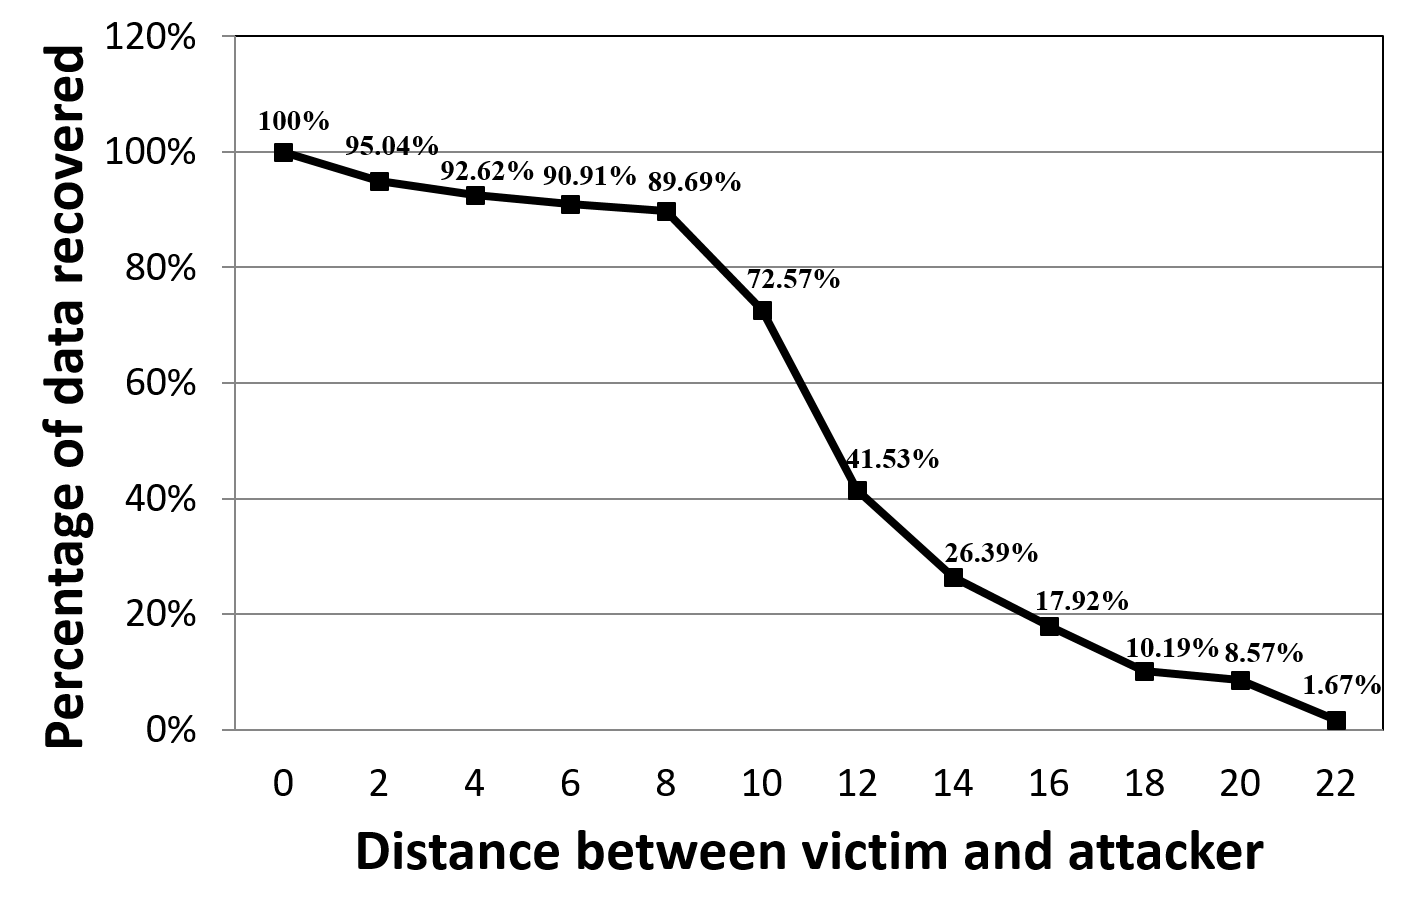
\includegraphics[scale=0.3]{recovereddata.png}
        \caption{The percentage graph of the EEG data being recovered \emph{vs.} the distance between the attacker and the victim. The $y$-axis is the percentage of data being recovered over the ground-truth data, while the $x$-axis is the distance in meters. %As shown in the graph, more than 90\% of the data can be recovered within 6 meters. When the distance increases to 8 meters, 89.69\% can be recovered; when the distance increases to 12 meters, the percentage of the recovered data drops to 41.53\%; and when it gets to 14 meters, the percentage drops to 26.39\%. If the distance increases to more than 20 meters, the percentage of recovered data drops to under 10\%.
        }
        \label{fig:recovereddata}
\end{figure}

\subsection{Effectiveness of the Inference Attack}
In order to evaluate our RCNN learning model, we need to have data for training and testing. Gathering data by ourselves is a tough and time-consumming task which involves recruiting volunteering, puchasing devices, setting up testing environments, and so on. Fortunately, NeuroSky published a large dataset publicly available on Kaggle for research~\cite{neuroskydata}, which contains 9,959 pieces of data collected by 30 volunteers. Each volunteer wore a NeuroSky headset constantly collecting the participant's EEG data for different tasks. Each data record contains a piece of reduced-featured EEG data with 11 features: signal poorness level, attention meter, meditation meter, and the 8 types of EEG waveforms as described in section~\ref{sec:background}. Even though taking raw voltage data into consideration may ameliorate the inference results, many apps do not request for the raw data by setting \texttt{enableRawOutput} to be true, meaning that it is not always possible for an attacker to retrieve the raw voltage data. Therefore, we only take these 11 features into our analysis since all these 11 features can be obtained by an attacker through our attacks, either from raw-packet format or JSON format as demonstrated in section~\ref{sec:framework}. There are 9 activities a participant may work on: reading instructions, blinking, seeing colors, solving math problems, listening to music, getting ready for next task, relaxing, thinking of an item, and watching videos. Each piece of data completely defines an activity. Echo back to our RCNN model, we have $n=9959$, $k=11$ and $m=9$.\\
%
\indent To evaluate the effectiveness of our model, we compared the prediction results by our model with those of other 11 most widely-used and well-known machine learning classifiers: SVM, Guassian Bayes, Bernoulli Bayes, Multinomial Bayes, K-nearest neighbors (KNN), decision tree, random forest, multi-layer perceptron (MLP), adaboost, quadratic discriminant analysis, and logistic regression. In a traditional statistical context, cross-validation is widely adopted for verifying the effectiveness of a learning model. However, in deep learning, it is a known fact that cross-validation should be avoided  since it is mostly suitable for small-sized datasets~\cite{deepcrossvalid}. In each simulation trial, we randomly chose 1,000 pieces of data for testing and used the rest for training, and applied each of the 12 algorithms for prediction; we repeated this procedure for 50 times and calculated the average prediction accuracies for reach classification algorithm. The results are reported in table~\ref{tbl:inferacc}. One can see that our RCNN model has an average accuracy of 70.55\%, which far exceeds those of all other popular classifiers. Note that we conducted the simulation study when 10\% and 20\% of the test data were dropped and obtained exactly the same results. This is reasonable as i) the training data is not affected as an adversary can collect training data from all possible channels and ii) each piece of data completely defines one activity.

\indent Note that we also tried to compare our inference model against the learning models in the NeuroSky BCI apps. \textcolor{blue}{We read the descriptions as well as reversely engineered the NeuroSky BCI apps and found that all the BCI apps used the internal model provided directly by the Thinkgear framework. We further analyzed and found that Thinkgear framework three inferred data, meditaion meter, attention meter and blink strength. Meditation meter and attention meter are served as input features for our learning model, therefore it has nothing to learn under our setting. As for blink detection, the Thinkgear framework infers a strength level (an integer) on how strong a person blinks while our model predicts whether a user is constantly blinking or doing other tasks such as solving math problems. All in all, our model is not comparable to the inference model leveraged by Thinkgear framework.}

\begin{table}[]
\centering
\caption{Inference accuracies of different classifiers.}
\label{tbl:inferacc}
\begin{tabular}{cc}
\hline
                       & \begin{tabular}[c]{@{}c@{}}Accuracy\end{tabular}  \\ \hline
Random Guess           & 11.11\%                                                                  \\ \hline
SVM                    & 29.59\%                                                                  \\ \hline
KNN                    & 10.35\%                                                                 \\ \hline
Gaussian Bayes         & 25.92\%                                                                  \\ \hline
Bernoulli Bayes        & 24.44\%                                                                 \\ \hline
Multinomial Bayes      & 10.17\%                                                                
\\ \hline
Decision Tree          & 24.94\%                                                                  \\ \hline
Random Forest          & 30.72\%                                                                  \\ \hline
MLP                    & 17.41\%                                                                  \\ \hline
Adaboost               & 28.79\%                                                                  \\ \hline
Quadratic Discriminant & 24.14\%                                                                  \\ \hline
Logistic Regression    & 27.61\%                                                                  \\ \hline
Our RCNN Model         & 70.55\%                                                                 \\ \hline
\end{tabular}
\end{table}



%Moreover, since data as we can see in figure~\ref{fig:recovereddata}, when the distance increases 8 meters, approximately 10\% of the data are lost; and when it gets to 10 meters, approximately 20\% data are lost. Therefore, we also consider the cases when 10\% and 20\% of the testing data are lost.
%%%%%%%%%%%%%%%%%%%%%%%%%%%%%%%%%%%%%%%%%%%%%%%%%
%As a result, the average prediction accuracy of our model reaches 70.55\%, 69.86\% and 69.77\%, respectively for full testing data, 10\% testing data loss and 20\% testing data loss. The performance of all classifiers are shown in table~\ref{tbl:inferacc}.

%\begin{table*}[]
%\centering
%\caption{Inference accuracies of different classifiers. % based on full training data, 10\% testing data loss and 20\% testing data loss. As we can see, our model can achieve a prediction accuracy as high as 70.55\%.
%}
%\label{tbl:inferacc}
%\begin{tabular}{cccc}
%\hline
%                       & \begin{tabular}[c]{@{}c@{}}Accuracy\\ (Full Testing Data)\end{tabular} & \begin{tabular}[c]{@{}c@{}}Accuracy\\ (10\% Testing Data Loss)\end{tabular} & \begin{tabular}[c]{@{}c@{}}Accuracy\\ (20\% Testing Data Loss)\end{tabular} \\ \hline
%Random Guess           & 11.11\%                                                                 & 11.11\%                                                                      & 11.11\%                                                                      \\ \hline
%SVM                    & 29.59\%                                                                 & 28.66\%                                                                      & 29.35\%                                                                      \\ \hline
%KNN                    & 10.35\%                                                                 & 10.17\%                                                                      & 10.09\%                                                                      \\ \hline
%Gaussian Bayes         & 25.92\%                                                                 & 25.92\%                                                                      & 26.02\%                                                                      \\ \hline
%Bernoulli Bayes        & 24.44\%                                                                 & 24.45\%                                                                      & 24.47\%                                                                      \\ \hline
%Multinomial Bayes      & 10.17\%                                                                 & 9.88\%                                                                      & 9.94\%                                                                       \\ \hline
%Decision Tree          & 24.94\%                                                                 & 24.88\%                                                                      & 24.43\%                                                                      \\ \hline
%Random Forest          & 30.72\%                                                                 & 30.32\%                                                                      & 30.03\%                                                                      \\ \hline
%MLP                    & 17.41\%                                                                 & 17.01\%                                                                      & 17.04\%                                                                      \\ \hline
%Adaboost               & 28.79\%                                                                 & 28.79\%                                                                      & 28.70\%                                                                      \\ \hline
%Quadratic Discriminant & 24.14\%                                                                 & 24.23\%                                                                      & 24.15\%                                                                      \\ \hline
%Logistic Regression    & 27.61\%                                                                 & 27.86\%                                                                      & 27.54\%                                                                      \\ \hline
%Our RCNN Model         & 70.55\%                                                                 & 69.86\%                                                                      & 69.77\%                                                                      \\ \hline
%\end{tabular}
%\end{table*}

